\documentclass[a4paper,twoside,notitlepage,
% draft,
11pt,
% fleqn
]{amsart}
\usepackage[margin=1in]{geometry}
\usepackage{tikz}
\usepackage{pdfpages}
\usetikzlibrary{shapes.geometric,positioning}
\newtheorem{theorem}{Theorem}[section]
% \newtheorem{lemma}[theorem]{Lemma}

% \theoremstyle{definition}
% \newtheorem{definition}[theorem]{Definition}
% \newtheorem{example}[theorem]{Example}
\newtheorem{xca}[theorem]{Problem}

% \theoremstyle{remark}
% \newtheorem{remark}[theorem]{Remark}

% \numberwithin{equation}{section}

\makeatletter
\renewcommand{\section}{\@startsection
  {section}% name
  {1}% level
  {\z@}% indent (0pt)
  {1.5ex plus 1ex minus .2ex}% space above
  {1ex plus .2ex}% space below
  {\normalfont\bfseries}}% font style

\renewcommand{\subsection}{\@startsection
    {subsection}% name
    {2}% level
    {\z@}% indent
    {1.5ex plus 1ex minus .2ex}% space above
    {1ex plus .2ex}% space below
    {\normalfont\itshape}}% font style
\makeatother


\begin{document}
\title[Pascal's Triangle]{Session 1 - Building a Pascal's Triangle}
\author{Disha Kuzhively}
\address{\textit{International Centre for Theoretical Sciences - TIFR, Bangalore}}
\email{disha.jk@icts.res.in}
\urladdr{dishajk.github.io}
\date{\today}
\maketitle
\section{Overview}
In the first session will be to introduce students to Pascal's Triangle and encourage pattern recognition through hands-on construction, collaborative activities, and visual re-imaginings. Following is a rough outline of the session.
\subsection*{1. Warm-up}
Begin with a brief guided worksheet where students solve a few problems involving simple counting tasks, exponentiation, such as calculating powers of 2. This primes the students for recognizing patterns that will emerge in Pascal's Triangle.
\begin{xca}
  Maya brought home chocolates for her 6 children, Asha, Bindu, Chaitra, Divya, Esha, and Farah. She gave them to the youngest, Farah and asked her to distribute them among her siblings. Farah ate half of the chocolates and gave the rest to Esha and asked her to distribute them among her younger siblings. Esha did the same, ate half and gave the rest to Divya and so on. In the end, the oldest child Asha got only one chocolate. How many chocolates did Maya bring home?

  What if Maya had 7 children instead of 6, what would be the number of chocolates Maya would have brought home then?
\end{xca}

\begin{xca}
  Find the sum of \(1+2+4+8+\ldots+1024\).
\end{xca}
\begin{xca}
  Below is the map of the city showing Maya's house and VITM. Maya visits VITM taking the shortest possible route.
  
  How many such routes are there?



  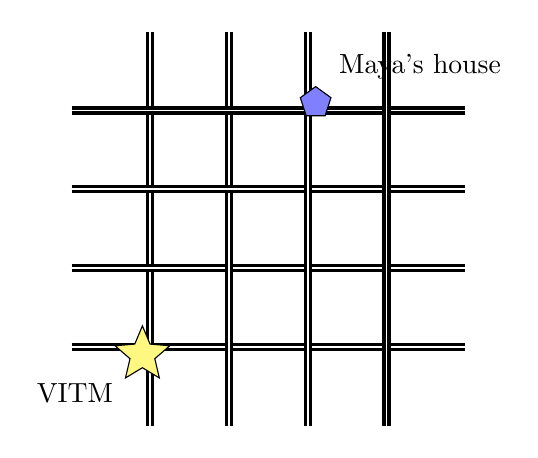
\begin{tikzpicture}
    \foreach \k in {0,1,...,3} {
      \draw[very thick, double] (0,\k) -- (5,\k);
      \draw[very thick, double] ({\k+1},-1) -- ({\k+1},4);
    }
    \node[star,star points=5,star point height=2mm,fill=yellow!50,draw] (m) at (0.9,-0.1) {};
    \node[below left=2pt of m] {VITM};
    \node[regular polygon,regular polygon sides=5,minimum size=2mm,fill=blue!50,draw] (n) at (3.1,3.1) {};
    \node[above right=2pt of n] {Maya's house};
  \end{tikzpicture}
\end{xca}
\begin{xca}
  Consider the layout below.

  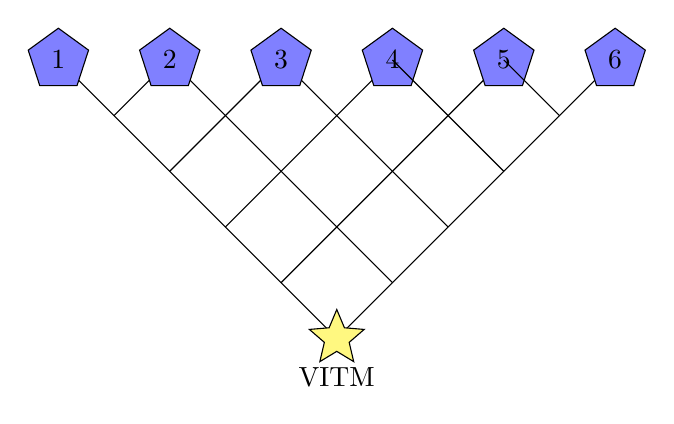
\begin{tikzpicture}
    \foreach \k in {0,1,...,5} {
        \pgfmathsetmacro{\h}{int(6 - \k)}
        \draw (135:\k)--++(45:{5-\k}) node[regular polygon,regular polygon sides=5,minimum size=2mm,fill=blue!50,draw] {\h};
        \draw (45:\k) --++ (135:{5-\k});
        }
    \node[star,star points=5,star point height=2mm,fill=yellow!50,draw] (m) at (0,0) {};
    \node[below=2pt of m] {VITM};
  \end{tikzpicture}

  The houses of 6 students who came to VITM today are marked in pentagons. How many routes can Student No. 5 take to return home. Keep in mind these students try to take the shortest possible routes. 
  
  Which of these students have the highest number of routes to return home?

\end{xca}
\subsection*{2. Building Pascal's Triangle}
Each student receives a worksheet to build the first several rows of Pascal's Triangle. Once completed, they are encouraged to observe and discuss patterns such as symmetry, alternating numbers, or diagonals resembling counting sequences (like natural numbers, figurate numbers, powers of 2, etc.).
\newpage
\thispagestyle{empty}
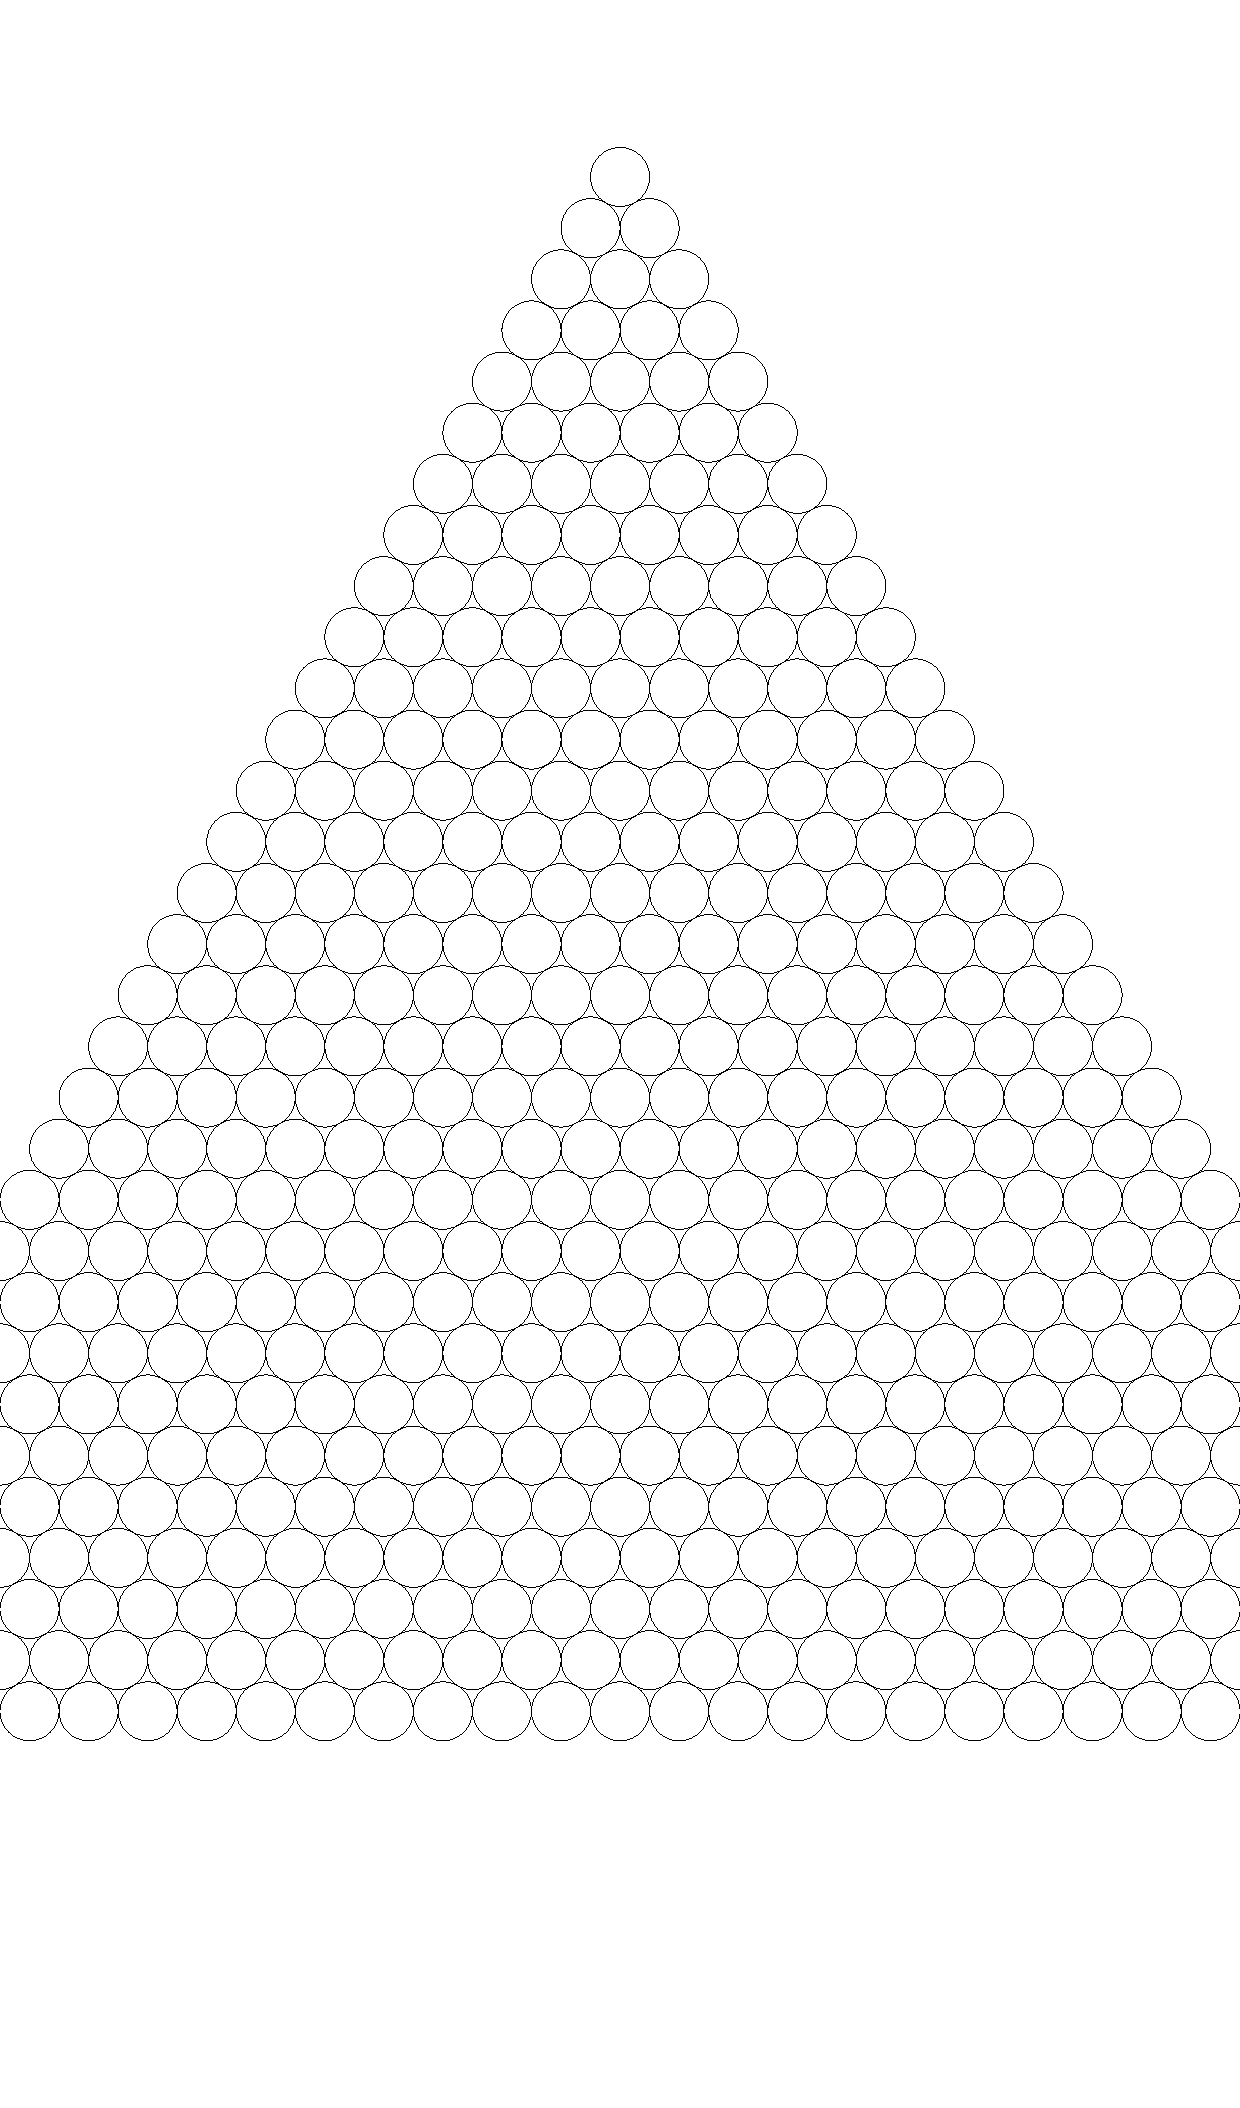
\includepdf[fitpaper=true]{pascalstriangle.pdf}
\newpage
Possible patterns that the students may notice:
\begin{enumerate}
  \item The sum of numbers in the nth row is \(2^n\).
  \item The sum of numbers in m+1 th row is twice the sum of numbers in mth row.
  \item All the rows are symmetric.
  \item For prime number \(p\), all numbers in the pth row are divisible by \(p\) except the first and the last one.
  \item Sum of squares of numbers in a row can be found along the bisector.
\end{enumerate}
\subsection*{3. Discussion and Pattern Exploration}
After constructing and observing the triangle, introduce Tartaglia's Rectangle. Ask students how do the patterns look now, are they easier or harder to see, which patterns remain, and which change?

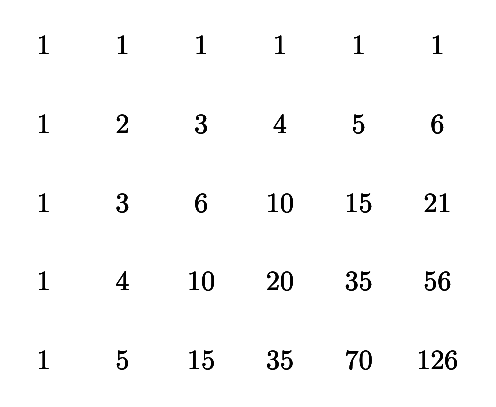
\begin{tikzpicture}
  \foreach \row in {0,1,...,5} {
    \foreach \col in {0,1,...,5}{
    \node at (\col,5) {1};
    \pgfmathsetmacro{\n}{int(\col+1)}
    \node at (\col,4) {{\n}};
    \pgfmathsetmacro{\na}{int((\col+2)*(\col+1)/2)}
    \node at (\col,3) {{\na}};
    \pgfmathsetmacro{\nb}{int((\col+2)*(\col+1)*(\col+3)/6)}
    \node at (\col,2) {{\nb}};
    \pgfmathsetmacro{\nc}{int((\col+1)*(\col+2)*(\col+3)*(\col+4)/24)}
    \node at (\col,1 ) {{\nc}};
    }
  %     \draw (135:\k)--++(45:{5-\k}) node[regular polygon,regular polygon sides=5,minimum size=2mm,fill=blue!50,draw] {\h};
  %     \draw (45:\k) --++ (135:{5-\k});
      }
  % \node[below=2pt of m] {VITM};
\end{tikzpicture}

Possible patterns that the students may notice:
\begin{enumerate}
  \item Each number is the sum of numbers in the row above starting from the leftmost to the number right above it.
  \item Each number is the sum of numbers in the column left starting from the topmost to the number preceding it.
  \item For any number \(a\) in the table, \(a-1\) is the sum of all the numbers in the reactangle bound by the column and row whose intersection is \(a\).
\end{enumerate}
\subsection*{4. Group Activity: Sierpinski Gasket}
Students use crayons to color the odd numbers in their triangle. Then, working in small groups, they assemble their triangles into a large Sierpinski Gasket on chart paper. Depending on the class size, this becomes a collective artwork for display.

How many odd numbers are there in the first 8 rows? 16 rows? 32 rows?

Fractals

How will the triangle look if we colored numbers that have remainder 1 when divided by 3 in green and numbers that have remainder 2 when divided by 3 in black?

\subsection*{5. Wrap-Up and Take-Home Exploration}
Introduce the lattice path problem: ``How many ways can you move from one corner of a grid to the opposite corner, moving only right or down?'' Encourage students to explore how Pascal's Triangle relates to this problem before the next session.

\begin{xca}

\end{xca}

\begin{xca}\footnote{1992 AIME I, Problem 4}
  In which row of Pascal's Triangle do three consecutive entries occur that are in the ratio $3: 4: 5$?
\end{xca}
\section*{Materials required}
\begin{enumerate}
    \item Crayons or any coloring material,
    \item masking tape or stapler,
    \item printout of worksheets
\end{enumerate}


\section*{Outcomes}
By the end of this session, students will be able to construct and understand Pascal's Triangle; recognize and describe patterns such as symmetry, row sums, diagonals, and powers of 2; and record their observations in their own words. They will explore how coloring the triangle modulo 2 gives rise to the Sierpinski gasket, providing a visual introduction to fractals. Students will also begin investigating path-counting in grid-like structures as a real-world application of Pascal's Triangle and develop curiosity about generalizing observed patterns into mathematical statements.

\section*{Subsequent Sections}
The design of Session 2 and later sessions will be informed by the students' responses and engagement in Session 1. These sessions will likely focus on figurate numbers and their appearance within Pascal's Triangle, the use of proof by induction to formally understand and verify the properties and patterns observed, and guiding students through the process of moving from empirical observation to a generalised mathematical statement.

This approach ensures that the workshop builds naturally on students' curiosity, and supports their transition from intuitive pattern recognition to structured mathematical reasoning.
\hrule
\end{document}